\documentclass[11pt,a4paper]{article}
\usepackage[utf8]{inputenc}
\usepackage{amsmath}
\usepackage{amssymb}
\usepackage{booktabs}
\usepackage{graphicx}
\usepackage{geometry}
\usepackage{microtype}
\usepackage{hyperref}
\usepackage{caption}
\usepackage{float}
\usepackage{titling} 

\setlength{\droptitle}{-5em}

\geometry{margin=1in}
\hypersetup{colorlinks=true, linkcolor=blue, citecolor=blue, urlcolor=blue}

\title{
    \textbf{\Large CSE 318: Artificial Intelligence Sessional} \\
    \Large Offline 1 Report: Performance Evaluation of Weighted $A^*$ Search using the Custom Heuristic on the 15-Puzzle
}

\author{
    \textbf{Shahriar Alam Patwary} \\
    Student ID: 2205062 \\
    \vspace{0.2em} \\
    \small Department of Computer Science and Engineering \\
    \small Bangladesh University of Engineering and Technology (BUET)
}
\date{} 

\begin{document}

\maketitle

\section{Introduction}
This report evaluates a custom heuristic design, \texttt{CornerLinearConflict}, implemented within a Weighted $A^*$ search framework to solve the 15-Puzzle ($4 \times 4$ sliding tile puzzle). Performance metrics are analyzed across ten distinct initial board configurations using four expansion weight parameters: $W \in \{1.0, 1.2, 2.0, 5.0\}$. 

\section{Heuristic Formulation}
The evaluated heuristic function, denoted as $h_{CLC}(n)$, is defined mathematically as follows:
\begin{equation}
    h_{CLC}(n) = h_M(n) + 2 \cdot \left( C_{LC}(n) + C_{corner}(n) \right)
\end{equation}
Where:
\begin{itemize}
    \item $h_M(n)$ is the standard Manhattan Distance baseline.
    \item $C_{LC}(n)$ represents the count of classical Linear Conflicts in the rows and columns.
    \item $C_{corner}(n)$ is the count of linear conflicts occurring strictly between tiles whose target goal destinations are one of the four grid corners.
\end{itemize}
\section{Initial Board Configurations}
\item Number of test cases: 10 randomly generated solvable configurations
\footnote{The puzzle configurations were generated using \texttt{https://15puzzle.netlify.app/}. The board arrays were extracted from screenshots with assistance from Google's Gemini.}
{\footnotesize % Makes the matrices more compact to guarantee they fit on page 1
\begin{align*}
\text{Case 1} &= \begin{pmatrix} 0 & 8 & 5 & 12 \\ 2 & 14 & 3 & 1 \\ 9 & 4 & 11 & 15 \\ 7 & 10 & 6 & 13 \end{pmatrix} & 
\text{Case 2} &= \begin{pmatrix} 4 & 11 & 8 & 2 \\ 0 & 9 & 12 & 15 \\ 7 & 5 & 1 & 13 \\ 6 & 3 & 10 & 14 \end{pmatrix} &
\text{Case 3} &= \begin{pmatrix} 2 & 4 & 6 & 8 \\ 14 & 3 & 13 & 5 \\ 7 & 9 & 11 & 0 \\ 12 & 15 & 10 & 1 \end{pmatrix} \\
\text{Case 4} &= \begin{pmatrix} 4 & 12 & 3 & 7 \\ 11 & 0 & 1 & 5 \\ 8 & 13 & 2 & 6 \\ 10 & 15 & 9 & 14 \end{pmatrix} &
\text{Case 5} &= \begin{pmatrix} 4 & 8 & 10 & 13 \\ 11 & 6 & 1 & 9 \\ 7 & 12 & 15 & 2 \\ 5 & 0 & 14 & 3 \end{pmatrix} &
\text{Case 6} &= \begin{pmatrix} 9 & 3 & 15 & 1 \\ 10 & 14 & 0 & 4 \\ 13 & 2 & 7 & 5 \\ 6 & 11 & 8 & 12 \end{pmatrix} \\
\text{Case 7} &= \begin{pmatrix} 1 & 13 & 9 & 0 \\ 10 & 5 & 11 & 4 \\ 12 & 2 & 6 & 3 \\ 15 & 14 & 7 & 8 \end{pmatrix} &
\text{Case 8} &= \begin{pmatrix} 1 & 8 & 6 & 15 \\ 4 & 12 & 14 & 0 \\ 3 & 7 & 13 & 5 \\ 10 & 9 & 2 & 11 \end{pmatrix} &
\text{Case 9} &= \begin{pmatrix} 14 & 10 & 7 & 2 \\ 0 & 5 & 6 & 9 \\ 4 & 1 & 12 & 15 \\ 3 & 8 & 11 & 13 \end{pmatrix}
\end{align*}
\begin{equation*}
\text{Case 10} = \begin{pmatrix} 10 & 13 & 2 & 15 \\ 9 & 1 & 5 & 7 \\ 14 & 4 & 12 & 3 \\ 6 & 11 & 0 & 8 \end{pmatrix}
\end{equation*}
}
\section{Empirical Search Metrics}
Table \ref{tab:metrics} outlines the behavior of the search space across varying weight bounds.

\begin{table}[H]
\centering
\caption{Weighted $A^*$ Search Metrics across Configurations}
\label{tab:metrics}
\small
\begin{tabular}{lcrrr}
\toprule
\textbf{Configuration} & \textbf{Weight ($W$)} & \textbf{Moves} & \textbf{Nodes Explored} & \textbf{Runtime (ms)} \\
\midrule
Case 1 & 1.0 & 48 & 143,357 & 2,717.0 \\
       & 1.2 & 48 & 143,357 & 2,945.1 \\
       & 2.0 & 50 & 495 & 7.9 \\
       & 5.0 & 110 & 562 & 12.9 \\
\midrule
Case 2 & 1.0 & 49 & 74,885 & 1,388.7 \\
       & 1.2 & 49 & 74,885 & 1,426.4 \\
       & 2.0 & 61 & 1,192 & 36.9 \\
       & 5.0 & 93 & 463 & 8.3 \\
\midrule
Case 3 & 1.0 & 53 & 2,425,638 & 50,588.8 \\
       & 1.2 & 53 & 2,425,638 & 59,384.5 \\
       & 2.0 & 61 & 904 & 17.2 \\
       & 5.0 & 93 & 362 & 8.2 \\
\midrule
Case 4 & 1.0 & 50 & 35,498 & 700.3 \\
       & 1.2 & 50 & 35,498 & 629.9 \\
       & 2.0 & 66 & 1,105 & 21.8 \\
       & 5.0 & 102 & 1,070 & 21.4 \\
\midrule
Case 5 & 1.0 & 58 & 6,473,694 & 140,571.0 \\
       & 1.2 & 58 & 6,473,694 & 167,406.8 \\
       & 2.0 & 70 & 7,420 & 142.0 \\
       & 5.0 & 94 & 365 & 6.9 \\
\midrule
Case 6 & 1.0 & 45 & 107,906 & 2,483.5 \\
       & 1.2 & 45 & 107,906 & 2,316.8 \\
       & 2.0 & 51 & 792 & 14.4 \\
       & 5.0 & 51 & 86 & 1.9 \\
\midrule
Case 7 & 1.0 & 47 & 245,337 & 5,538.8 \\
       & 1.2 & 47 & 245,337 & 5,453.1 \\
       & 2.0 & 51 & 1,314 & 27.0 \\
       & 5.0 & 73 & 401 & 9.2 \\
\midrule
Case 8 & 1.0 & 50 & 110,953 & 2,403.6 \\
       & 1.2 & 50 & 110,953 & 2,794.2 \\
       & 2.0 & 68 & 10,351 & 223.7 \\
       & 5.0 & 92 & 1,816 & 39.5 \\
\midrule
Case 9 & 1.0 & 55 & 1,606,130 & 35,473.9 \\
       & 1.2 & 55 & 1,606,130 & 39,797.1 \\
       & 2.0 & 65 & 2,136 & 39.9 \\
       & 5.0 & 93 & 363 & 6.3 \\
\midrule
Case 10& 1.0 & 47 & 375,353 & 8,145.8 \\
       & 1.2 & 47 & 375,353 & 8,408.3 \\
       & 2.0 & 61 & 1,155 & 22.7 \\
       & 5.0 & 75 & 320 & 6.8 \\
\bottomrule
\end{tabular}
\end{table}

\newpage
\section{Experimental Visualizations and Analysis}

\begin{figure}[htbp]
    \centering
    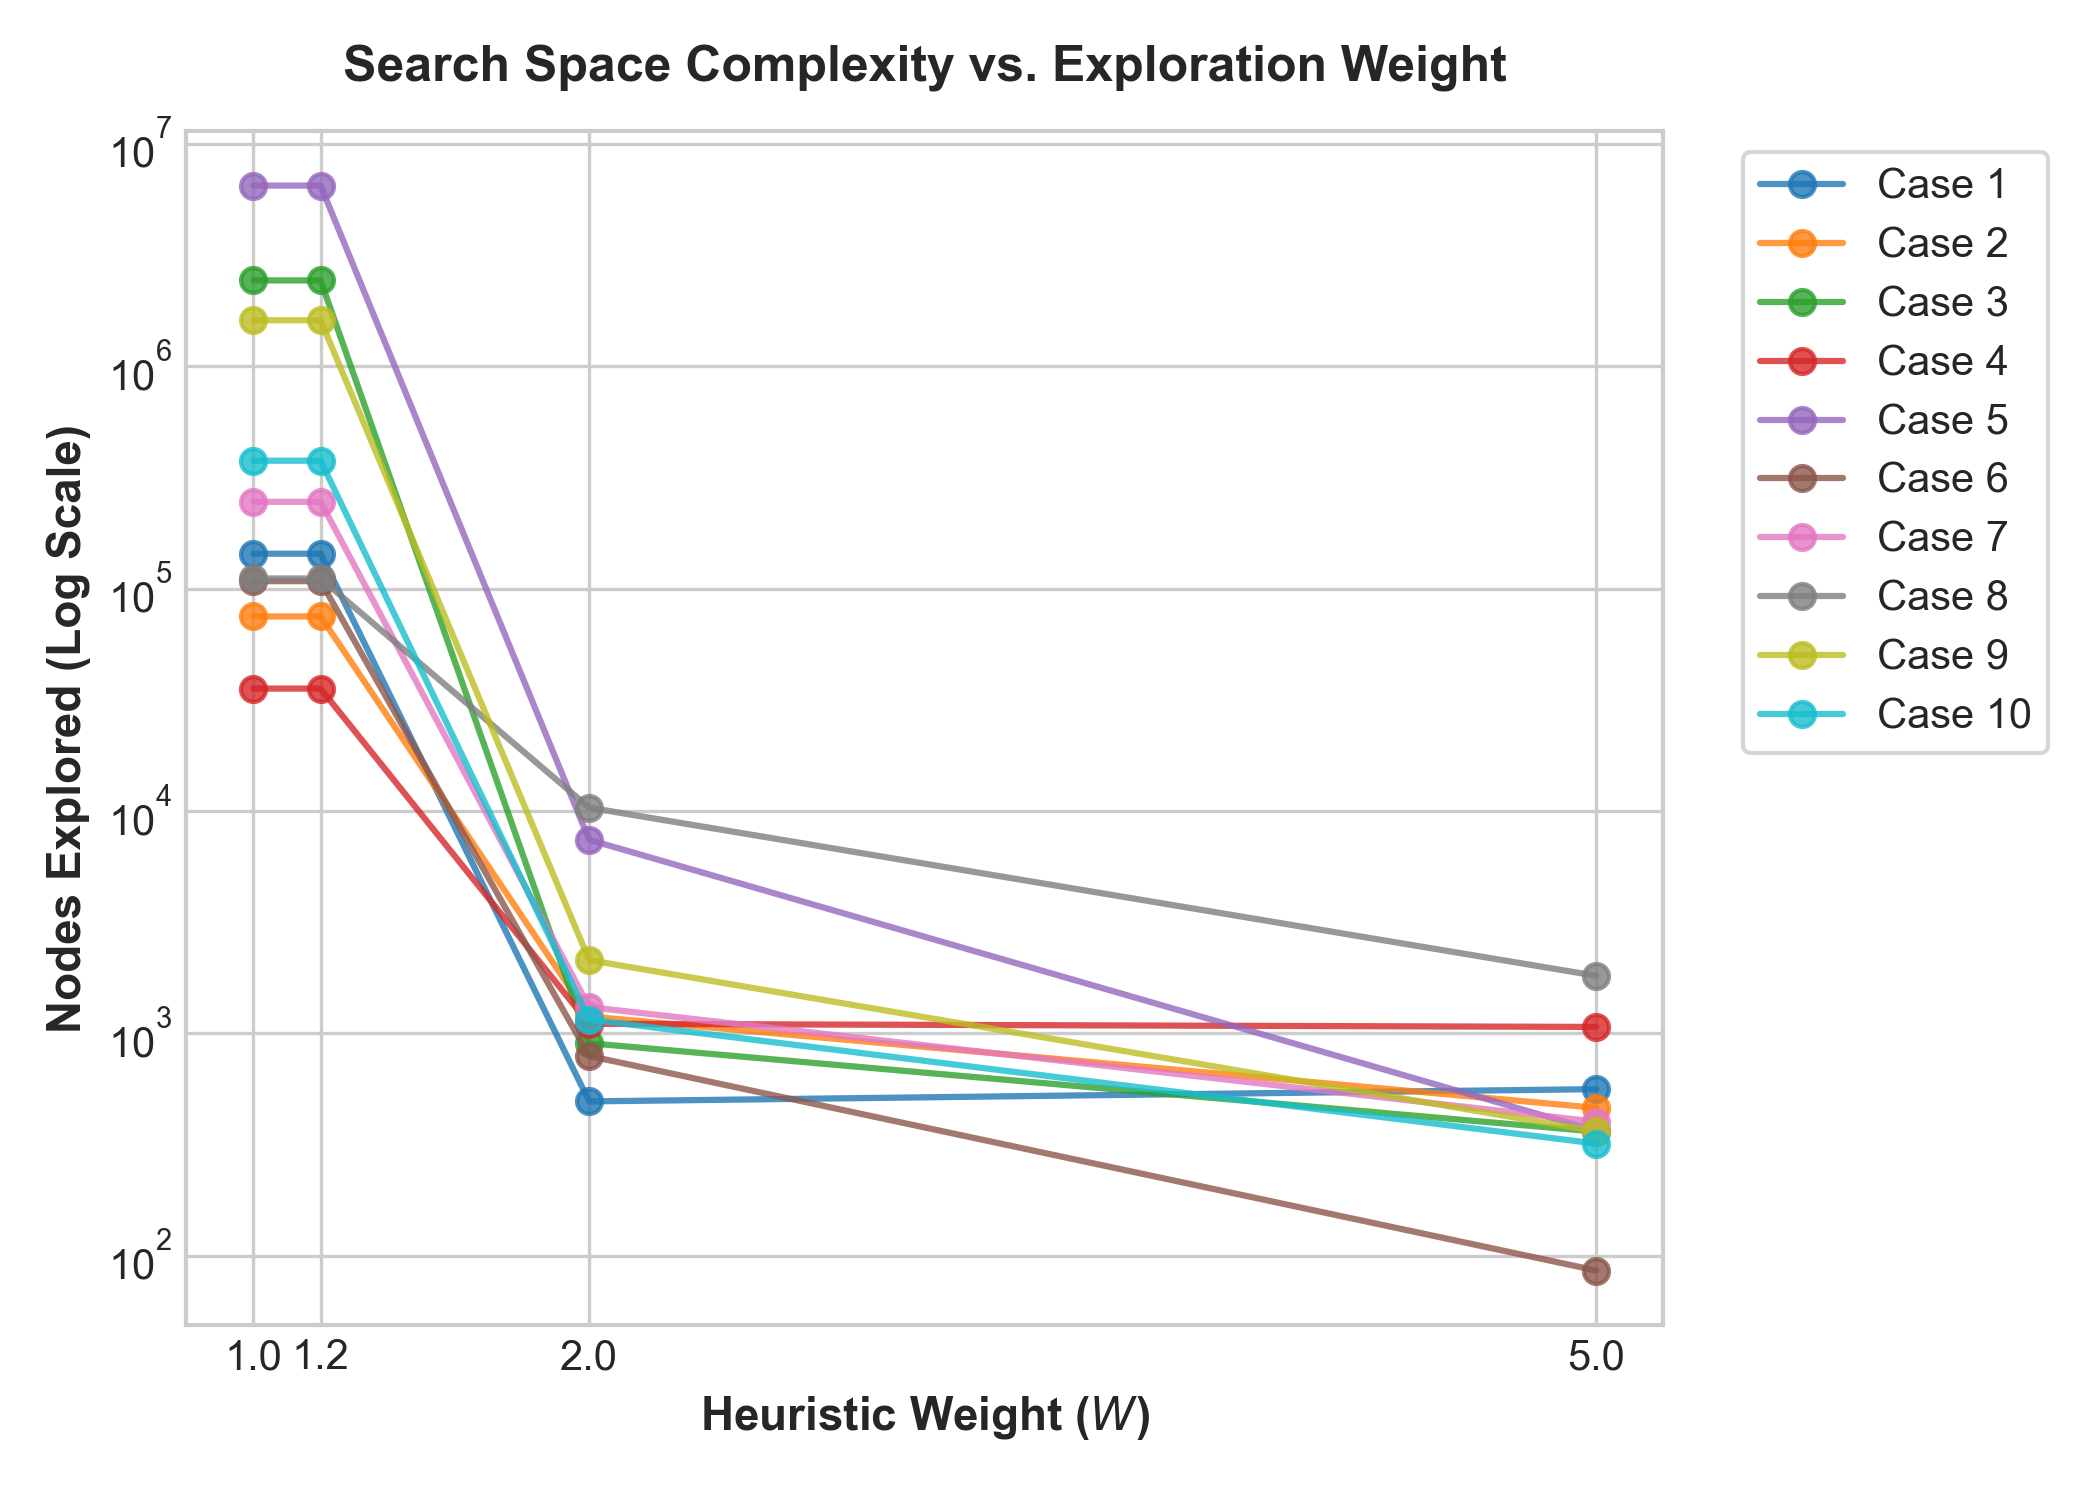
\includegraphics[width=0.68\textwidth]{nodes_vs_weight.png}
    \caption{Total Nodes Explored across configurations plotted against Heuristic Weight ($W$) using a logarithmic scale.}
    \label{fig:nodes_vs_weight}
\end{figure}

\begin{figure}[htbp]
    \centering
    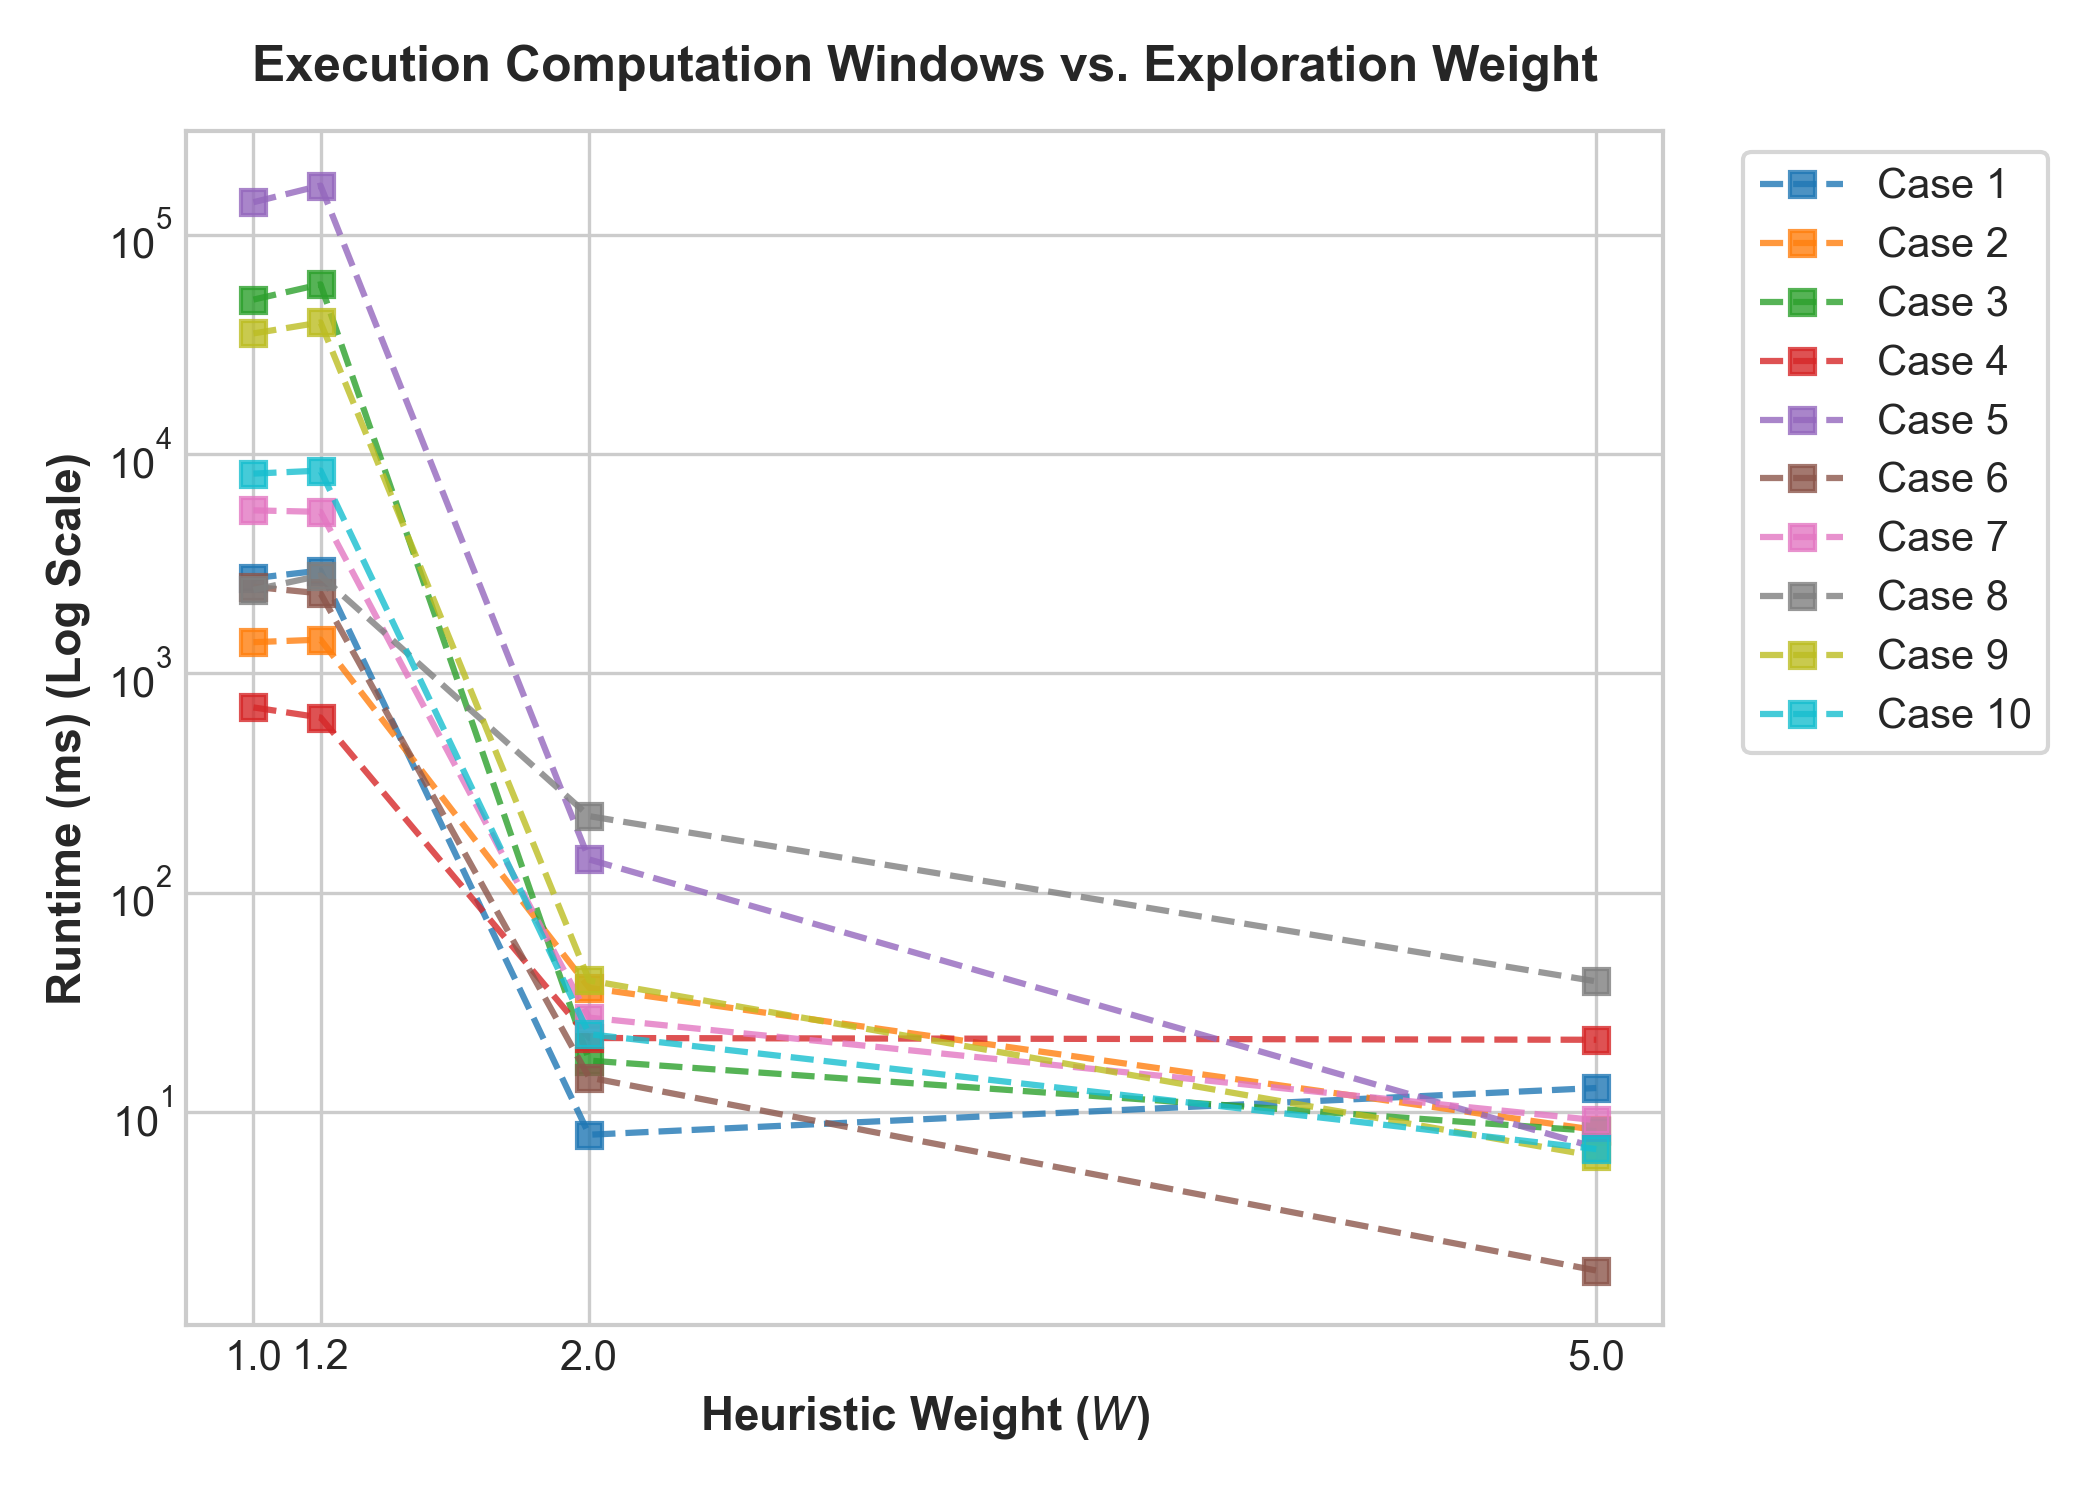
\includegraphics[width=0.68\textwidth]{runtime_vs_weight.png}
    \caption{Algorithm Execution Runtime (ms) across configurations plotted against Heuristic Weight ($W$) using a logarithmic scale.}
    \label{fig:runtime_vs_weight}
\end{figure}

\begin{figure}[htbp]
    \centering
    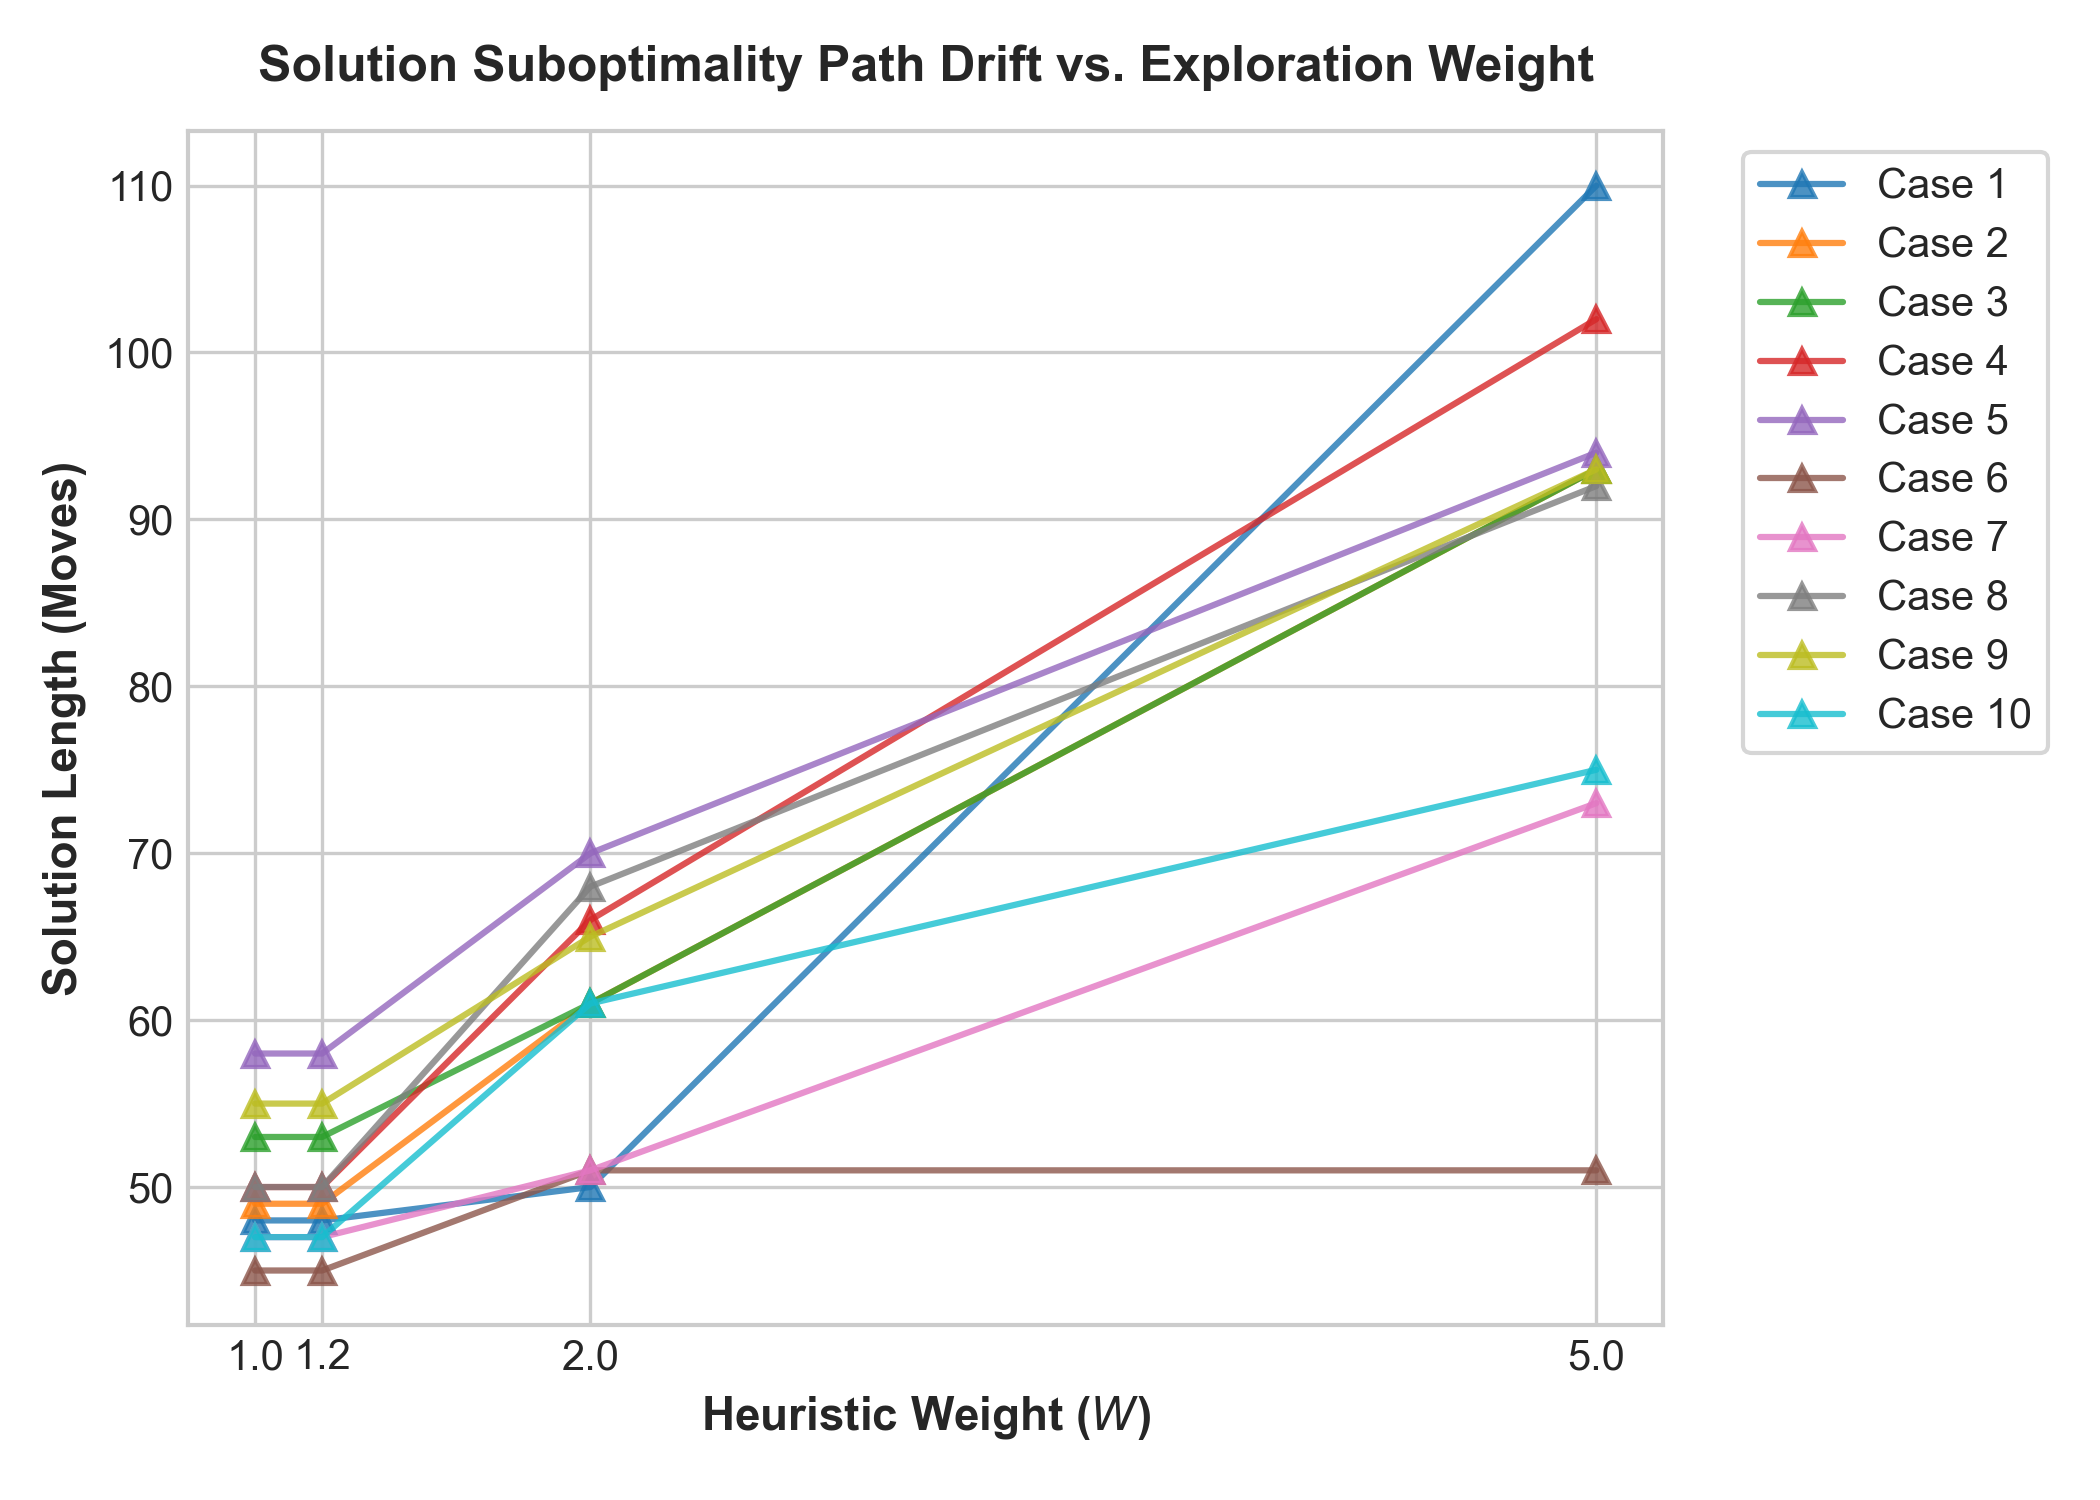
\includegraphics[width=0.68\textwidth]{moves_vs_weight.png}
    \caption{Total moves needed to solve puzzles across configurations plotted against Heuristic Weight ($W$).}
    \label{fig:nodes_explored_vs_weight}
\end{figure}
\newpage
\subsection{Key Performance Trends}
\begin{enumerate}
    \item \textbf{Heuristic Scale Insensitivity ($W=1.0$ vs $W=1.2$):} Across all test scenarios, the node expansion counts match exactly between $W=1.0$ and $W=1.2$. This occurs because the integer values generated by our inflated heuristic dominate the search evaluation equation $f(n) = g(n) + W \cdot h(n)$. Scaling $h(n)$ by a factor of 1.2 does not alter the relative processing sequence within the priority queue.
    \item \textbf{Exponential Decay of Search Volume ($W \ge 2.0$):} As $W$ escalates, the search strategy shifts towards a greedy best-first pattern. In Case 5, increasing the weight boundary from $1.0$ to $5.0$ reduces the explored state footprint from $6,473,694$ to a mere $365$ nodes—representing an execution efficiency return of over $99.99\%$.
    \item \textbf{Suboptimality Inflation:} The performance savings achieved by setting $W = 5.0$ introduce severe suboptimality. For instance, Case 1 expands from an optimal path of $48$ moves to a winding solution of $110$ moves.
\end{enumerate}

\end{document}